\section{Reševanje enačb}
\label{pogl:enacbe}


% - enačbe 4. stopnje (TEŽJE) --> Alhazen's problem (gl.\ članek od Vavšetiča in tudi~\cite[str.\ 137--139]{geometricconstructions})
% - enačbe 5. stopnje (TEŽJE)

Zapustimo deloma področje geometrije in si poglejmo, kako lahko s prepogibanjem papirja rešujemo enačbe z racionalnimi koeficienti.

Spomnimo se še, da smo origami-konstruktibilna števila definirali kot vsa števila, ki jih lahko s prepogibanjem konstruiramo preko na začetku dane abscine osi, izhodišča $(0,0)$ in točke $(1,0)$ in da lahko kar predpostavimo, da imamo dan celoten koordinatni sistem z abscisno in ordinatno osjo, izhodiščem ter enoto $1$ na obeh oseh (definicija~\ref{def:origami_konstruktibilnost}). V tej ravnini bomo konstruirali rešitve naših enačb, da pa bo pregibov čim manj in s tem preglednost večja, lahko pomožne točke in premice narišemo kar s svinčnikom (ker bi jih tako ali tako znali konstruirati s pregibi).

V tem poglavju si bomo pogledali, kako z origamijem na prefinjen način -- brez konstrukcije preko zgornjih petih operacij -- rešujemo enačbe druge, tretje, četrte in pete stopnje. Za vsak $n \in \{2, 3, 4, 5\}$ bomo reševali enačbo
$$ a_n x^n + a_{n-1} x^{n-1} + \ldots + a_2 x^2 + a_1 x + a_0 = 0, $$
kjer so $a_i \in \Q$ za vsak $i \in \{1, 2, \ldots, n\}$ in $a_n \neq 0$. Ker bo $i$ največ $5$, bomo namesto koeficientov $a_i$ uporabljali kar črke $a, b, c, d, e, f$.

Začnimo z najbolj osnovno, t.\ j.\ linearno enačbo. Enačba $ax + b = 0$ ima rešitev $x = -b/a$, ki je racionalno število in po izreku~\ref{izr:origami_konstruktibilnost} origami-konstruktibilno. Če bi želeli rešitev konstruirati brez računanja. bi lahko v ravnini prepognili premico $y = ax + b$ (konstruiramo npr.\ točki (0, b) in (1, a+b) in skoznju prepogneno premico) in njeno presečišče z abscisno osjo je iskana rešitev. Vendar je ta konstrukcija bolj zamudna kot direktna konstrukcija izračunane rešitve.

Za rešitev kvadratne enačbe lahko uporabimo znanje iz podpoglavja~\ref{podpogl:evkl_konstruktibilnost} -- vemo, da lahko z neoznačenim ravnilom in šestilom konstruiramo natanko števila oblike $a + b\sqrt{r}$, kjer so $a, b, r \in \Q$. Take oblike je tudi splošna rešitev kvadratne enačbe z racionalnimi koeficienti in ker lahko ta števila konstruiramo tudi z origamijem, lahko preko kvadratne formule najprej izračunamo realni rešitvi in ju nato s prepogibanjem papirja preko operacij seštevanja, odštevanja, množenja, deljenja in korenjenja konstruiramo (izrek~\ref{izr:origami_konstruktibilnost}). Zanima pa nas, ali jih je mogoče konstruirati tudi brez predhodnega računanja.

Ključno vlogo bosta v nadaljevanju odigrali origami operaciji~\ref{op:O6} in~\ref{op:O7}. Prva nam hkrati s konstrukcijo tangente na parabolo določi tudi točko na paraboli, skozi katero je pregib tangenten na stožnico, to pa je ekvivalentno reševanju kvadratne enačbe. Druga pa s konstrukcijo skupne tangente na dve paraboli omogoča reševanje kubične enačbe, saj imata paraboli v evklidski ravnini največ tri skupne tangente (glej~\cite[str.\ 149--150]{geometricconstructions}) \textcolor{red}{(dej tle še neko potrdilo, zakaj je skupna tangenta ekvivalentna reševanju kubične enačbe)}. Znano je tudi, da lahko reševanje kvartične enačbe prevedemo na reševanje kubične ali celo kvadratne (\textcolor{red}{dej vir, npr.\ uni članek v zavihku z enačbami}), zato nam origami rešuje tudi enačbe četrte stopnje. To je že skoraj 100 let nazaj odkrila italijanska matematičarka Margherita P.\ Beloch, ki je s tem odkrila pravo moč prepogibanja papirja.

Za rešitev enačbe pete stopnje pa bomo morali prekršiti pravilo o enkratnih prepogibih. Namreč \textcolor{red}{(preveri)} ni načina, kako s po enimi pregibom naenkrat konstruirati rešitev, \textcolor{red}{DOKONČAJ -- Alperin, Lang, Lucero so neki delali, 2-fold origami ???}

\subsection{Kvadratna enačba}
\label{podpogl:kvadratna_enacba}

Rešujemo enačbo oblike
$$ a x^2 + b x + c = 0, $$
kjer so $a, b, c \in \Q$ in velja $a \neq 0$.  Njeni splošni rešitvi sta
$$ x_{1,2} = \frac{-b \pm \sqrt{b^2 - 4ac}}{2a},$$ vendar so konstrukcije vseh teh števil časovno potratno, zato iščemo hitrejši način reševanja.

Postopek, ki si ga bomo pogledali v nadaljevanju, predpostavlja $a = 1$. Ker je vodilni koeficient neničeln, lahko z njim enačbo delimo in pri tem še vedno dobimo racionalne koeficiente, zato lahko predpostavko brez škode za splošnost sprejmemo. Nova oblika enačbe je tako
\begin{equation}
    \label{eq:spl_kv_en}
    x^2 + bx + c = 0.
\end{equation}
Predpostavimo, da ima enačba dve različni realni rešitvi oz.\ da je diskriminanta enačbe pozitivna, t.\ j.\ $D = b^2 - 4c > 0$. Če realnih ničel ni, o origami konstrukciji rešitev namreč nima smisla razpravljati. Če je rešitev ena, je podana kot $x = -b/2$, kar je origami-konstruktibilno število in se ga lahko takoj konstruira.

Enačba~\ref{eq:spl_kv_en} nam poda pokončno parabolo $y = x^2 + bx + c$ z vodoravno premico vodnico in dvema ničlama, ki sta rešitvi naše enačbe. Iščemo absciso presečišča parabole z abscisno osjo.

Zopet se bomo poslužili dosedanjega znanja o operaciji~\ref{op:O6}. Ta nam s pregibom skozi dano točko $B$, ki točko $A$ položi na premico $a$, konstruira tangento na parabolo z goriščem v točki $A$ in premico vodnico $a$.

Naša parabola je z enačbo seveda natančno določena. Ideja iskane konstrukcije rešitev enačbe je določiti tako točko $B$ (najlažje kar na osi parabole), da bi nam izvedba operacije~\ref{op:O6} podala tangento na parabolo ravno v njeni ničli. Želeni pregib mora potekati skozi točko $B$ in gorišče $A$ položiti na tisto točko $A'$ na premici vodnici $a$, ki ima enako absciso kot ničla parabole. (gl.\ sliko~\ref{fig:tockaB_in_O6}). Taka točka $B$ je z osjo parabole in katerokoli izmed ničlama (zaradi simetrije) natanko določena.

\begin{figure}[h]
    \centering
    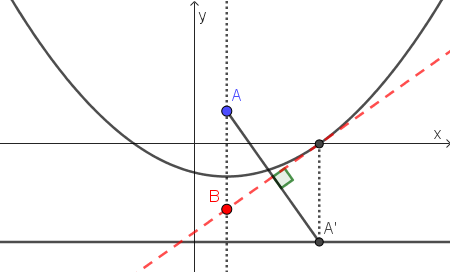
\includegraphics[width=0.5\textwidth]{images/kvadratna_enacba/tockaB_in_O6.png}
    \caption[Iskanje točke $B$]{Operacijo~\ref{op:O6} skozi iskano točko $B$ poda rešitev kvadratne enačbe.}
    \label{fig:tockaB_in_O6}
\end{figure}

Edina nevarnost, da ta konstrukcija ne bo delovala, je možnost, da točka $B$ kdaj ne bo origami-konstruktibilna točka. Zato sedaj izračunajmo njene koordinate in se prepričajmo, da se to nikoli ne bo zgodilo.

Najprej iz dane enačbe parabole določimo njeno gorišče $A$ in premico vodnico $a$. Spomnimo se, da iz enačbe parabole oblike
$$ (x - x_0)^2 = 2p(y - y_0) $$
takoj razberemo koordinati gorišča $(x_0, y_0)$ in enačbo premice vodnice $y = y_0 - p$. V našem primeru enačbo $y = x^2 + bx + c$ preoblikujemo v
$$ \left(x-\left(-\frac{b}{2}\right)\right)^2 = 2 \cdot \frac{1}{2} \left(y - \left(c - \frac{b^2}{4}\right)\right). $$
S tem sta gorišče $A$ in premica vodnica $a$ določena:
$$ A\left(-\frac{b}{2}, c - \frac{b^2 - 1}{4}\right) \text{ in } a: y = c - \frac{b^2 + 1}{4}. $$

Naj bo $t$ ena izmed rešitev enačbe~\ref{eq:spl_kv_en}. Na premici $a$ z $A'$ označimo točko z absciso $t$. Poiščimo enačbo pregiba, ki gorišče $A$ položi v točko $A'$. Ta pregib bo tangenten na parabolo ravno v njeni ničli, njegovo presečišče z osjo parabole $ x = -b/2 $ pa nam bo določilo točko $B$.

Koeficient nosilke daljice $AA'$ je $ - 1/(2t + b)$, torej je koeficient pregiba $k = 2t + b$. Pregib je po konstrukciji tangenten na parabolo v ničli $(t, 0)$, torej je njegova enačba
$$ y = (2t + b)(x - t) = (2t + b)x - 2t^2 - bt = (2t + b)x - t^2 + c. $$
Pri tem smo upoštevali, da velja $t^2 + bt + c = 0$. Presečišče pregiba in osi parabole je tako točka $B$ z absciso $ x = -b/2 $ in ordinato
$$ y = (2t + b)\left(-\frac{b}{2}\right) - t^2 + c = - t^2 - tb + c - \frac{b^2}{2} = c + c - \frac{b^2}{2} = 2c - \frac{b^2}{2}.$$
Obe koordinati sta racionalni, torej je točka $B$ konstruktibilna točka. Ker leži na osi parabole, nam poda obe rešitvi enačbe -- pregiba sta si simetrična glede na os. Povzemimo sedaj postopek konstrukcije rešitve kvadratne enačbe~\ref{eq:spl_kv_en}:
\begin{enumerate}
    \item V koordinatnem sistemu označimo gorišče $A\left(-\frac{b}{2}, c - \frac{b^2}{4} + \frac{1}{4}\right)$, premico vodnico $a: y = c - \frac{b^2}{4} - \frac{1}{4}$ in točko $B(-\frac{b}{2}, 2c - \frac{b^2}{2})$.
    \item Z operacijo~\ref{op:O6} naredimo pregib skozi točko $B$, ki točko $A$ položi na premico $a$ (če je diskriminanta enačbe pozitivna, sta možna pregiba dva).
    \item Skozi sliko točke $A$ naredimo vertikalen pregib in abscisa njegovega presečišča z abscisno osjo je ničla dane enačbe.
\end{enumerate}

\textbf{Primer:} Poiščimo rešitve enačbe $x^2 - x - 1 = 0$. Določimo obe točki in premico: $A(\frac{1}{2}, -1)$, $B(\frac{1}{2}, -\frac{5}{2})$ in $a: y = -\frac{3}{2}.$. Opravimo operacijo~\ref{op:O6} in označimo presečišče abscisne osi in pravokotnice nanjo skozi sliko točke $A$. Če smo bili pri pregibanju natančni, dobimo presečišči pri $x_{1,2} = \frac{1 \pm \sqrt{5}}{2}$ (gl.\ sliko v~\cite[str.\ 37]{hull2020}).

To še zdaleč ni edini postopek za reševanje kvadratne enačbe. Kot še en lep primer Hull v\~cite[str.\ 38]{hull2020} navaja Lillovo metodo, dokaz pa prepušča bralcu. Ta metoda je tudi zgled, kako lahko najprej najdemo evklidsko konstrukcijo rešitev kvadratne enačbe in jo nato preobrazimo v origami konstrukcijo -- saj že vemo, da lahko s prepogibanjem papirja konstruiramo vse in še več, kar se da z evklidskim orodjem.

\subsection{Kubična enačba}

Rešujemo enačbo oblike
$$ a x^3 + b x^2 + c x + d = 0, $$
kjer so $a, b, c, d \in \Q$ in velja $a \neq 0$.

Operacija~\ref{op:O6} nam je preko konstrukcije tangente na parabolo pomagala rešiti kvadratno enačbo. Spomnimo se, da je Belocheva to v 30-ih letih prejšnjega stoletja nadgradila z operacijo~\ref{op:O7}, ki nam konstruira skupno tangento na dve paraboli hkrati. Po njej jo tudi imenujemo \emph{Belochin pregib}. Z njim je kot prva odkrila resnično moč origami konstrukcij, a je žal trajalo več kot pol stoletja, da so matematiki začeli ceniti njeno odkritje. Le redki so njeno delo poznali in ji tudi pripisali avtorstvo.

Belocheva je s svojim pregibom oblikovala postopek, s katerim lahko preko origamija rešujemo kubične enačbe. Postopek temelji na Lillovi genialni metodi iskanja ničel poljubnih polinomov z realnimi koeficienti, ki si jo bomo v naslednjem razdelku podrobneje pogledali.

\subsubsection{Lillova metoda}

Njen avtor je avstrijski inženir Eduard Lill, ki jo je l.\ 1867 opisal v svojem članku~\cite{lill1867}. Gre za inovativen postopek, ki je v svoji osnovi čisto enostaven. Imejmo poljuben polinom $ p(x) = a_n x^n + a_{n-1} x^{n-1} + \ldots + a_2 x^2 + a_1 x + a_0 $ z realnimi koeficienti in iščemo njegove realne ničle, če obstajajo. Lill je iz njegovih koeficientov s sledečim postopkom v ravnini ustvaril enolično pot. Običajno se za njeno konstrukcijo uporablja figuro želve, ki nam kaže, v katero smer se premika pa tudi kam je usmerjena.

Na začetku želvo postavimo v koordinatno izhodišče $O$ tako, da gleda v pozitivno smer $x$-osi. Želva najprej v to smer prehodi razdaljo, enako koeficientu $a_n$. Nato se obrne za $90^\circ$ v nasprotno smer urinega kazalca in prehodi naslednjo razdaljo $a_{n-1}$. To ponovi za vsak koeficient polinoma in po prehojeni razdalji $a_0$ se ustavi v neki točki $T$ (slika~\ref{fig:primera_zelve}). Če je kateri od koeficientov negativen, želva hodi ritensko (primer (b) na sliki~\ref{fig:primera_zelve} za koeficiente $a_3, a_2$ in $a_0$), v primeru ničelnega koeficienta pa obstoji na mestu in se samo obrne. S potjo želve dobimo lomljeno črto iz največ $n+1$ daljic, ki jih brez škode označujmo kar z njihovimi ``pripadajočimi'' koeficienti.

\begin{figure}[h]
    \centering
    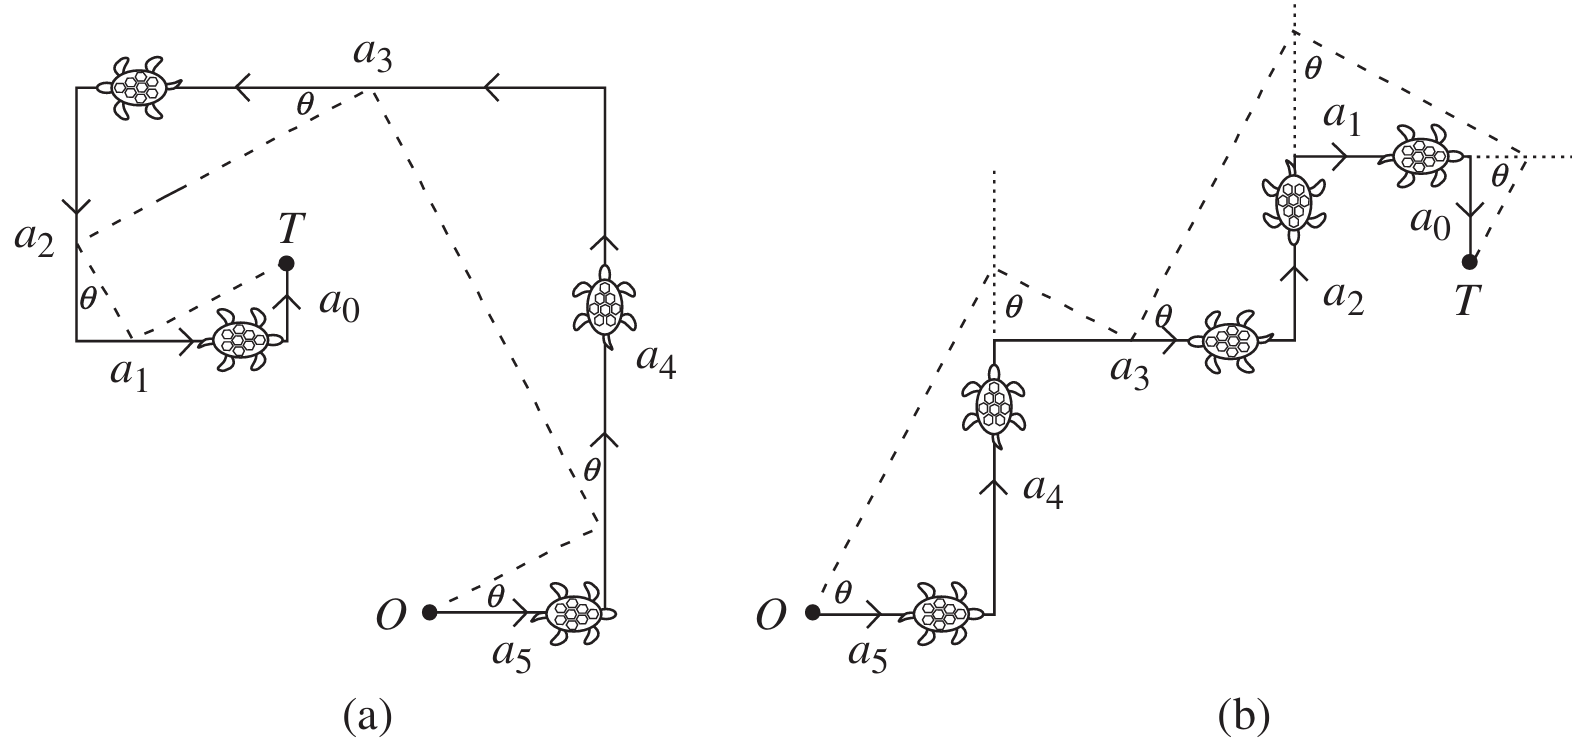
\includegraphics[width=0.9\textwidth]{images/kubična enačba/primera_zelvine_poti.png}
    \caption[Primera želvine poti]{Primera želvine poti za polinoma pete stopnje. Vzeto iz~\cite[str.\ 311]{hull2011}.}
    \label{fig:primera_zelve}
\end{figure}

Sedaj se v izhodišče $O$ postavimo še mi in z laserskim žarkom poskusimo zadeti želvo v točki $T$. Žarek najprej usmerimo daljico $a_{n-1}$, od katere se odbije v daljico $a_{n-2}$, od te v daljico $a_{n-3}$ in tako naprej. (slika~\ref{fig:primera_zelve}). Pri tem upoštevamo troje:
\begin{itemize}
    \item laserski žarek ne upošteva odbojnega zakona in se od daljice vedno odbije pod kotom $90^\circ$, zato so vpadni koti žarka na vse daljice med seboj enaki in prav tako to velja za odbojne kote;
    \item žarek se lahko odbije tudi od nosilke daljice;
    \item vsakič sta možni dve smeri odboja -- na isto stran daljice (oz.\ njene nosilke) ali skoznjo -- izberemo pa tisto, ki nam omogoči, da sploh lahko zadenemo naslednjo daljico.
\end{itemize}
ecimo, da smo zmogli zadeti želvo. Kot, ki ga v točki $O$ oklepata laserski žarek in abscisna os, označimo z $\theta$.

\begin{trditev}
    $x_{\theta} = - \tan \theta$ je ničla polinoma $p(x)$.
\end{trditev}

\begin{dokaz}
    Vzemimo primer, ko so vsi koeficienti polinoma $p(x)$ pozitivni. Želvina pot je v tem primeru sestavljena iz $n+1$ daljic, pot laserskega žarka (ki se vedno odbije od daljice in ne njene nosilke) pa iz $n$ daljic. Slednje so ravno hipotenuze pravokotnih trikotnikov. Za vsako od njih je nasprotna kateta kota $\theta$ del daljice $a_i$, priležno kateto pa označimo z $y_i$ ($ n \geq i \geq 1$). dobimo
    \begin{align*}
        y_n &= \tan \theta \cdot a_n = - x a_n \\
        y_{n-1} &= \tan \theta \cdot (a_{n-1} - y_n) = - x (a_{n-1} + x a_n) = - (a_{n-1} x + a_n x^2)\\
        y_{n-2} &= \tan \theta \cdot (a_{n-2} - y_{n-1}) = - x (a_{n-2} + a_{n-1} x + a_n x^2) = - (a_{n-2} x + a_{n-1} x^2 + a_n x^3) \\
        &\vdots \\
        y_1 &= - (a_1 x + a_2 x^2 + \ldots + a_{n-1} x^{n-1} + a_n x^n).
    \end{align*}
    V zadnji enakosti desno stran premaknimo na levo in upoštevamo $y_1 = a_0$. Dobimo ravno $p(x) = 0$, torej je $x = - \tan \theta$ res ničla tega polinoma.

    Primer negativnih koeficientov:~\cite[str.\ 36]{zore2022}.

    Primer ničelnih koeficientov: isto kot prej, samo se spusti $y_i$ za tisti $i$, za katerega je $a_i = 0$. (\textcolor{red}{???})
\end{dokaz}

Če pod nobenim kotom $\theta$ ne moremo zadeti želve, je polinom $p(x)$ brez realnih ničel.

Pojavi se nam vprašanje, kako določiti kot $\theta$. Za polinom tretje stopnje je Belocheva preko svojega pregiba našla zelo preprosto rešitev, ki si jo bomo sedaj pogledali.

\subsubsection{Belochin kvadrat}

Imejmo dani točki $A$ in $B$ ter premici $r$ in $s$. Z origamijem konstruirajmo kvadrat $WXYZ$, kjer oglišče $X$ leži na premici $r$, njegovo sosednje oglišče $Y$ pa na premici $s$. Velja še, da točka $A$ leži na stranici $WX$ (ali njeni nosilki), točka $B$ pa na stranici $ZY$ (ali njeni nosilki, slika~\ref{fig:beloch_kvadrat}).

\begin{figure}[h]
    \centering
    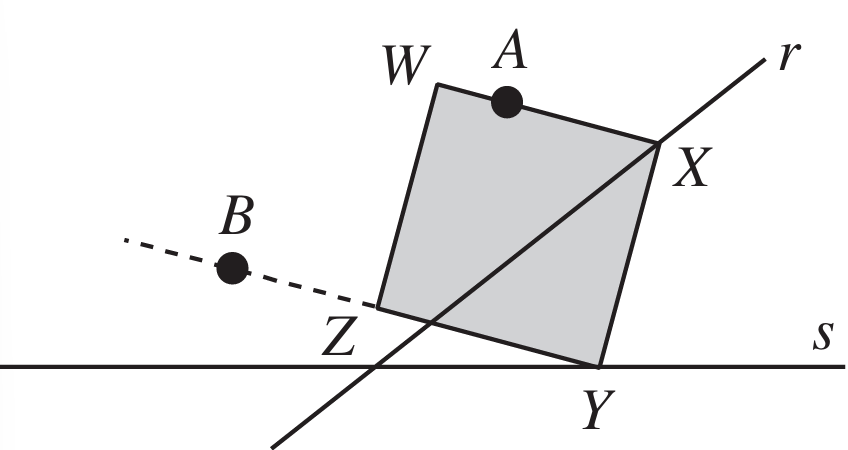
\includegraphics[width=0.4\textwidth]{images/kubična enačba/beloch_kvadrat.png}
    \caption[Belochin kvadrat]{Belochin kvadrat. Vzeto iz~\cite[str.\ 309]{hull2011}.}
    \label{fig:beloch_kvadrat}
\end{figure}

Belocheva je iznašla naslednji postopek, ki nam konstruira ta kvadrat:
\begin{itemize}
    \item Najprej konstruiramo premico $r'$, ki je vzporedna premici $r$ in od nje enako oddaljena kot točka $A$, tako da premica $r$ leži med točko $A$ in premico $r'$. Na enak način premici $s$ konstruiramo njeno vzporednico $s'$ (slika~\ref{fig:beloch_kvadrat_konstrukcija} levo). To konstrukcijo opravimo s prepogibi iz operacije~\ref{op:O5}, zrcaljenja točke čez premico ter ponovne uporabe operacije~\ref{op:O5}. Zaradi preglednosti seveda dopuščamo, da namesto zrcaljenja preprosto prepognemo po premici in s svinčnikom označimo sliko točke.
    \item Nato opravimo Belochin pregib, ki točko $A$ slika v točko $A'$ na premici $r'$, točko $B$ pa v točko $B'$ na premici $s'$ (slika~\ref{fig:beloch_kvadrat_konstrukcija} na sredi).
    \item Naj bo točka $X$ središče daljice $AA'$ in točka $Y$ središče daljice $BB'$. Ker je pregib simetrala teh dveh daljic $AA'$ in $BB'$, sta njuni središči po konstrukciji\footnote{Gledamo lahko dva podobna pravokotna trikotnika s skupnim ogliščem v točki $A$ (oz.\ $B$), enega dvakrat večjega od drugega} ravno presečišči pregiba s premicama $r$ in $s$ (slika~\ref{fig:beloch_kvadrat_konstrukcija} desno).
    \item Daljica $XY$ -- ena izmed stranic kvadrata -- je po konstrukciji pravokotna na daljici $AX$ in $BY$, zato samo še določimo točki $W$ in $Z$ na daljicah ali njunih nosilkah in tako dobimo Belochin kvadrat.
\end{itemize}

\begin{figure}[h]
    \centering
    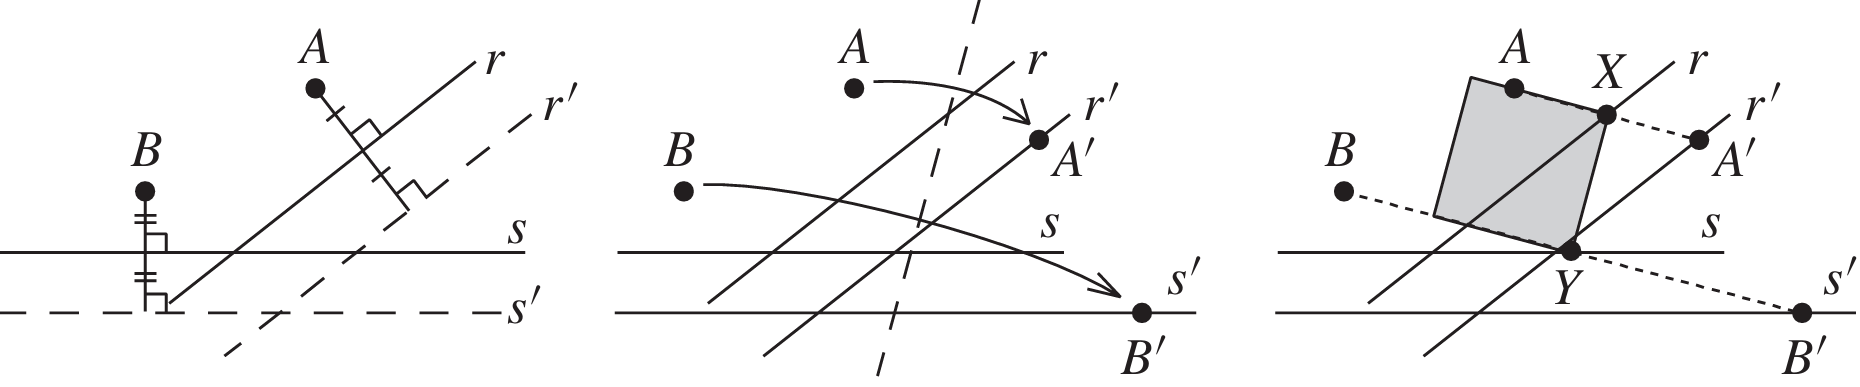
\includegraphics[width=0.95\textwidth]{images/kubična enačba/beloch_kvadrat_konstrukcija.png}
    \caption[Konstrukcija Belochinega kvadrata]{Konstrukcija Belochinega kvadrata z origamijem. Vzeto iz~\cite[str.\ 310]{hull2011}.}
    \label{fig:beloch_kvadrat_konstrukcija}
\end{figure}

\subsubsection*{Konstrukcija $\sqrt[3]{2}$ z Belochinim kvadratom}
\label{podpogl:beloch_kvadrat_koren}

Preden ravno naučeno znanje uporabimo za reševanje kubičnih enačb, si še na hitro poglejmo, kako lahko tudi z Belochinim kvadratom rešimo starogrški problem podvojitve kocke.

Za premico $r$ vzemimo ordinatno os, za premico $s$ pa abscisno os. Določimo še $A = (-1,0)$ in $B = (0, -2)$. Vzporednici sta torej $r': x = 1$ in $s': y = 2$. Belochin pregib seka premico $r$ v točki $X$, premico $s$ pa v točki $Y$ (slika~\ref{fig:beloch_koren}). Z $O$ označimo koordinatno izhodišče in opazimo podobne pravokotne trikotnike $OAX$, $OXY$ in $OYB$. Z upoštevanjem $|AO| = 1 $ in $|OB| = 2$ dobimo sledeča razmerja:
$$ \frac{|OX|}{|AO|} = \frac{|OY|}{|OX|} = \frac{|OB|}{|OY|} \Longrightarrow |OX| = \frac{|OY|}{|OX|} = \frac{2}{|OY|}, $$
iz česar sledi
$$ |OX|^3 = |OX| \cdot \frac{|OY|}{|OX|} \cdot \frac{2}{|OY|} = 2 \Longrightarrow |OX| = \sqrt[3]{2}. $$

\begin{figure}[h]
    \centering
    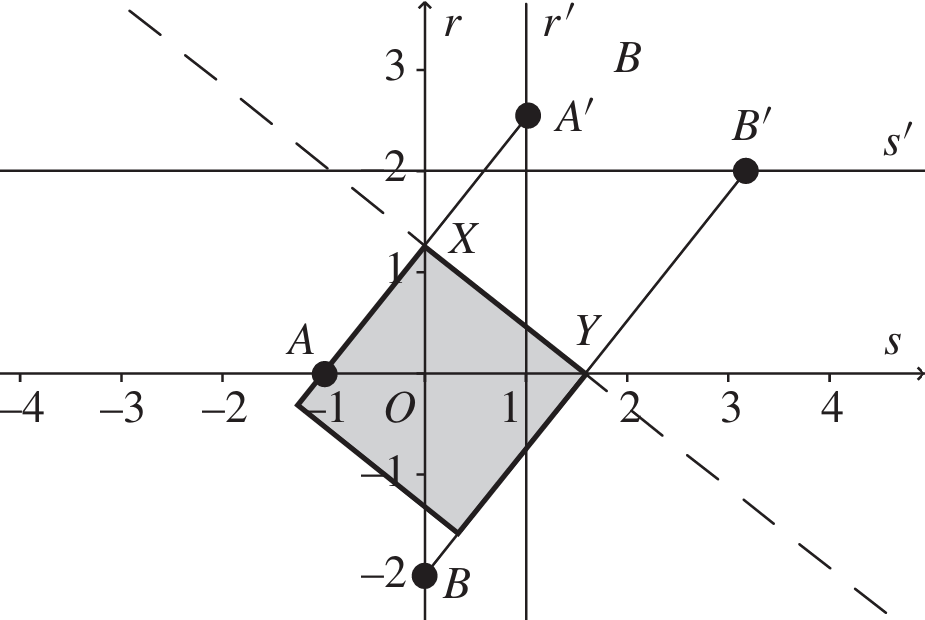
\includegraphics[width=0.5\textwidth]{images/kubična enačba/beloch_koren.png}
    \caption[Konstrukcija kubičnega korena števila dva]{Konstrukcija $\sqrt[3]{2}$ preko Belochinega kvadrata. Vzeto iz~\cite[str.\ 310]{hull2011}.}
    \label{fig:beloch_koren}
\end{figure}

Vidimo lahko, da je to enaka konstrukcija kot jo je 50 let kasneje neodvisno od Belocheve odkril G.\ Martin (razdelek~\ref{podpogl:podvojitev_kocke}), le da je za točko $B$ vzel točko $(0, -k)$ in s tem konstruiral dolžino $\sqrt[3]{k}$ za poljuben origami-konstruktibilen $k$.

\subsubsection{Reševanje enačbe po Lillovi metodi z Belochinim pregibom}

Za poljubno enačbo $a_3 x^3 + a_2 x^2 + a_1 x + a_0 = 0$ (\textcolor{red}{a daš koeficiente a, b, c, d? in da $A \neq 0$ Potem je treba tut na slikci spremenit.}) povežimo sedaj Lillovo metodo s primerno konstrukcijo Belochinega kvadrata, ki nam bo natančno določil kot $\theta$. Najprej konstruiramo želvino pot za polinom $p(x) = a_3 x^3 + a_2 x^2 + a_1 x + a_0$. V primeru neničelnih koeficientov je pot sestavljena iz štirih stranic, pot laserskega žarka pa iz treh.

Za točko $A$ vzemimo izhodišče $O$, za točko $B$ pa končno točko $T$. Premica $r$ naj bo nosilka daljice $a_2$, premica $s$ pa nosilka daljice $a_1$. Ko si določimo premici $r'$ in $s'$ ter opravimo Belochin pregib, dobimo, kot običajno, na njegovih presečiščih s premicama $r$ in $s$ točki $X$ in $Y$. Ker velja $ AX \perp XY \perp BY $, je to iskana pot laserskega žarka, ki se odbija pod pravim kotom in zadene želvo. Kot $theta$ je kot, ki ga oklepata daljici $a_3$ in $AX$ (slika~\ref{fig:beloch_kubicna_resitev}).

\begin{figure}[h]
    \centering
    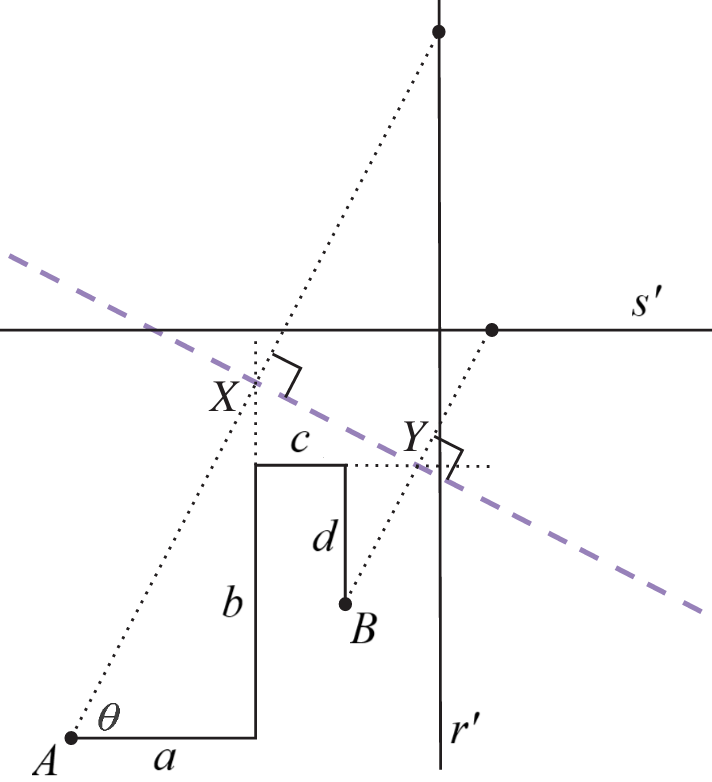
\includegraphics[width=0.4\textwidth]{images/kubična enačba/beloch_kubicna_resitev.png}
    \caption[Lillova metoda z Belochinim kvadratom]{Konstrukcija želvine poti za Lillovo metodo preko Belochinega kvadrata. Vzeto in preurejeno iz~\cite[str.\ 313]{hull2011}.}
    \label{fig:beloch_kubicna_resitev}
\end{figure}

Ker imata dve paraboli največ tri skupne tangente, obstajajo največ trije prepogibi, ki točki $A$ in $B$ zaporedoma položijo na premici $r'$ in $s'$. Kolikor je možnih pregibov, toliko realnih rešitev ima naša enačba.

\opomba{V resnici nikoli do sedaj nismo potrebovali konstruirati celega kvadrata; potrebovali smo le stranico $XY$ in dejstvo, da je pregib pravokoten na daljici $AX$ in $BY$.}

\textcolor{red}{Kaj je v primeru, ko je kakšen koeficient ničeln?}

\textcolor{red}{Daj kakšen primer. Eden s samimi pozitivnimi koeficienti, eden z negativnim in ničelnim?}

\subsubsection{Alperinova rešitev}

\textcolor{red}{a čmo tudi to?} (gl.\ Hull 2020, hull2013 str.\ 78 spodej) - prevedba kubične enačbe na kvadratno al neki tazga.

\subsection{Kvartična enačba}

\emph{Abel-Ruffinijev izrek}, ki temelji na Galoisovi teoriji, pravi, da je štiri najvišja stopnja polinomske enačbe, za katere rešitve obstaja splošna formula v radikalih, t.\ j.\ izrazih, ki vsebujejo korenjenje~\cite{mrinal2019}. Splošna formula na sliki~\ref{fig:kvarticna_formula} \textcolor{red}{lepše povej, nas odvrne haha}

\begin{figure}[h]
    \centering
    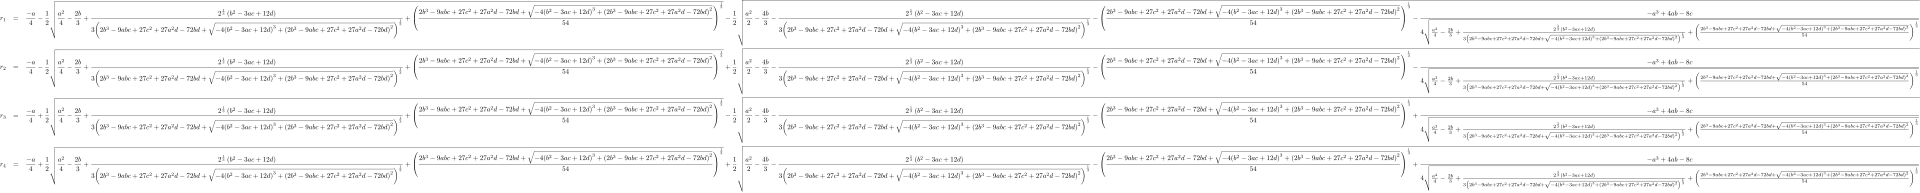
\includegraphics[width=0.95\textwidth]{images/quartic_formula.png}
    \caption[Kvartična formula]{Splošna formula za rešitev enačbe četrte stopnje.}
    \label{fig:kvarticna_formula}
\end{figure}

Kot smo omenili že na začetku poglavja, se da kvartično enačbo z uvedbami novih spremenljivk prevesti na kubično. Načinov je več, gl.\ \cite{wikiquartic}.

% kot redukcija na kubično ali kvadratno??
% citiram od začetka poglavja: Znano je tudi, da lahko reševanje kvartične enačbe prevedemo na reševanje kubične ali celo kvadratne, zato nam origami rešuje tudi enačbe četrte stopnje.

\subsection{Kvintična enačba}

\textcolor{red}{Če boš to obdelala v poglavju MULTIFOLD, potem spremeni na začetku tega poglavja, da bomo gledali samo enačbo do 4.\ stopnje.}